\documentclass[10pt,a4paper]{article}
\usepackage[utf8]{inputenc}
\usepackage[T1]{fontenc}
\usepackage{polski}
\usepackage[margin=2.2cm,headheight=14pt]{geometry}
\usepackage{amsmath,amssymb}
\usepackage{graphicx}
\usepackage{booktabs}
\usepackage{array}
\usepackage{fancyhdr}
\usepackage{lastpage}
\usepackage{hyperref}
\usepackage{caption}

\hypersetup{
    colorlinks=true,
    linkcolor=black,
    urlcolor=blue,
    citecolor=black
}

\pagestyle{fancy}
\fancyhf{}
\fancyhead[L]{\small Mateusz Portka}
\fancyhead[R]{\small Algorytmy Geometryczne --- Laboratorium 1}
\fancyfoot[C]{\small Strona \thepage\ z \pageref{LastPage}}
\renewcommand{\headrulewidth}{0.4pt}
\renewcommand{\footrulewidth}{0pt}

\begin{document}

% --- METRYCZKA I STRONA TYTUŁOWA ---
\thispagestyle{empty}
\noindent
\begin{tabular}{ll}
\textbf{Imię i nazwisko:} & Mateusz Portka \\
\textbf{Data wykonania:} & 20 października 2026 r. \\
\textbf{Kierunek / Przedmiot:} & Informatyka / Algorytmy Geometryczne \\
\textbf{Numer ćwiczenia:} & Laboratorium 1
\end{tabular}

\vspace{2.5cm}

\begin{center}
    {\LARGE \textbf{Sprawozdanie z Laboratorium 1}}\\[0.4cm]
    {\Large \textbf{Podstawowe predykaty geometryczne}}\\[0.2cm]
    {\normalsize Badanie stabilności numerycznej testu orientacji punktu względem prostej\\
    w arytmetyce zmiennoprzecinkowej IEEE 754}
\end{center}

\vspace{2.5cm}

\tableofcontents
\newpage

% --- SEKCJA 1 ---
\section{Dane techniczne i środowisko testowe}
Wszystkie symulacje numeryczne, obliczenia wyznaczników oraz pomiary wydajności czasowej przeprowadzono w następującym środowisku sprzętowo-programowym:
\begin{itemize}
    \item \textbf{Platforma sprzętowa:} Apple MacBook Air (Apple M4, 10 rdzeni: 4 Performance + 6 Efficiency)
    \item \textbf{Pamięć operacyjna:} 24 GB zunifikowanej pamięci RAM (Unified Memory)
    \item \textbf{System operacyjny:} macOS 26.2 (kompilacja 25C56)
    \item \textbf{Środowisko i interpreter:} Python 3.13.2 (64-bit), środowisko wirtualne \texttt{.venv}
    \item \textbf{Zastosowane biblioteki zewnętrzne:}
    \begin{itemize}
        \item \texttt{numpy} (wersja 2.5.4) --- struktury tablicowe i procedura algebry \texttt{np.linalg.det}
        \item \texttt{pandas} (wersja 3.0.6) --- analiza tabelaryczna i agregacja wyników eksperymentów
        \item \texttt{matplotlib} (wersja 3.11.2) --- generowanie wieloosiowych wykresów wysokiej rozdzielczości
        \item \texttt{time.perf\_counter} --- precyzyjny licznik czasu o rozdzielczości nanosekundowej
    \end{itemize}
\end{itemize}

% --- SEKCJA 2 ---
\section{Podstawy teoretyczne}

\subsection{Problem orientacji punktu względem prostej}
Podstawowym predykatem geometrycznym w przestrzeni dwuwymiarowej jest określenie położenia badanego punktu $C = (x_c, y_c)$ względem zorientowanej prostej wyznaczonej przez dwa punkty bazowe $A = (x_a, y_a)$ oraz $B = (x_b, y_b)$.

O orientacji decyduje wartość wyznacznika $D$ z uwzględnieniem progu tolerancji $\varepsilon \ge 0$:
\begin{equation}
\text{Kwalifikacja orientacji} = \begin{cases}
\text{Lewo (L)} & \text{gdy } D > \varepsilon \\
\text{Prawo (R)} & \text{gdy } D < -\varepsilon \\
\text{Na prostej (ON)} & \text{gdy } |D| \le \varepsilon
\end{cases}
\end{equation}

Geometrycznie oznacza to, że gdy poruszamy się wzdłuż prostej od punktu $A$ do punktu $B$, dodatnia wartość wyznacznika wskazuje na położenie punktu $C$ po naszej lewej stronie, ujemna --- po prawej, natomiast wartość bliska zeru ($|D| \le \varepsilon$) świadczy o współliniowości punktów.

\subsection{Porównywane metody obliczeniowe}
Do wyznaczenia wartości $D$ zastosowano cztery procedury obliczeniowe:
\begin{enumerate}
    \item \texttt{custom\_3x3} --- autorska implementacja wyznacznika macierzy $3 \times 3$ (formuła Sarrusa),
    \item \texttt{custom\_2x2} --- autorska implementacja wyznacznika macierzy różnic współrzędnych $2 \times 2$,
    \item \texttt{numpy\_3x3} --- biblioteczna funkcja \texttt{np.linalg.det} dla macierzy $3 \times 3$,
    \item \texttt{numpy\_2x2} --- biblioteczna funkcja \texttt{np.linalg.det} dla macierzy różnic $2 \times 2$.
\end{enumerate}

\subsection{Wpływ arytmetyki IEEE 754 i rola parametru $\varepsilon$}
W komputerowej reprezentacji liczb zmiennoprzecinkowych mantysa ma ograniczoną pojemność bitową: format \texttt{float32} zapewnia około 7 dziesiętnych cyfr znaczących, natomiast \texttt{float64} około 16 cyfr.

Gdy operujemy na współrzędnych o dużych rzędach wielkości (np. $10^{14}$), odejmowanie bliskich sobie liczb prowadzi do zjawiska \emph{eliminacji katastrofalnej}. Wiodące cyfry ulegają wyzerowaniu, a wynik zostaje zdominowany przez błędy zaokrągleń, co w formacie \texttt{float32} skutkuje powstaniem fałszywego zera maszynowego. Wprowadzenie progu tolerancji $\varepsilon$ pozwala odróżnić rzeczywiste odchylenia geometryczne od naturalnych fluktuacji numerycznych maszyny.

\newpage

% --- SEKCJA 3 ---
\section{Realizacja ćwiczenia i zbiory testowe}

\subsection{Prosta testowa $AB$}
Prosta bazowa została zdefiniowana przez dwa punkty: $A = (-1.0, 0.0)$ oraz $B = (1.0, 0.1)$. Jej postać kierunkowa przyjmuje postać:
\begin{equation}
y = 0.05x + 0.05
\end{equation}

\subsection{Specyfikacja zbiorów punktów}
W ramach laboratorium wygenerowano pięć niezależnych zbiorów punktów:
\begin{itemize}
    \item \textbf{Zestaw A ($10^5$ punktów):} Rozkład jednostajny ciągły w obszarze $[-1000, 1000]^2$. Odpowiada typowym danym inżynierskim.
    \item \textbf{Zestaw B ($10^5$ punktów):} Rozkład jednostajny w skrajnym obszarze $[-10^{14}, 10^{14}]^2$, prowokujący błędy niedomiaru mantysy.
    \item \textbf{Zestaw C ($10^3$ punktów):} Punkty na okręgu o środku $S=(0,0)$ i promieniu $R=100$, wyznaczane równaniem $x = R\cos\theta, y = R\sin\theta$ dla $\theta \in [0, 2\pi)$.
    \item \textbf{Zestaw D --- wersja kierunkowa ($10^3$ punktów):} Punkty leżące matematycznie na prostej, generowane wzorem $y = 0.05x + 0.05$ dla $x \in [-1000, 1000]$.
    \item \textbf{Zestaw D --- wersja parametryczna ($10^3$ punktów):} Punkty generowane równaniem parametrycznym dla $t \in [-500, 500]$, co daje współrzędne $x = -1 + 2t$ oraz $y = 0.1t$.
\end{itemize}

\subsection{Parametry eksperymentów}
Każdy zestaw punktów przebadano dla pełnego iloczynu kartezjańskiego: 4 metody obliczeniowe, 2 typy precyzji (\texttt{float64}, \texttt{float32}) oraz 6 progów tolerancji $\varepsilon \in \{0, 10^{-14}, 10^{-12}, 10^{-10}, 10^{-8}, 10^{-6}\}$.

Łącznie wykonano 240 prób kwalifikacyjnych.

\newpage

% --- SEKCJA 4 ---
\section{Wyniki i analiza eksperymentalna}

\subsection{Wizualizacja wygenerowanych zbiorów danych}
Na Rysunku~\ref{fig:raw} przedstawiono rozkład przestrzenny punktów w czterech podstawowych zbiorach przed wykonaniem klasyfikacji.

\begin{figure}[htbp]
    \centering
    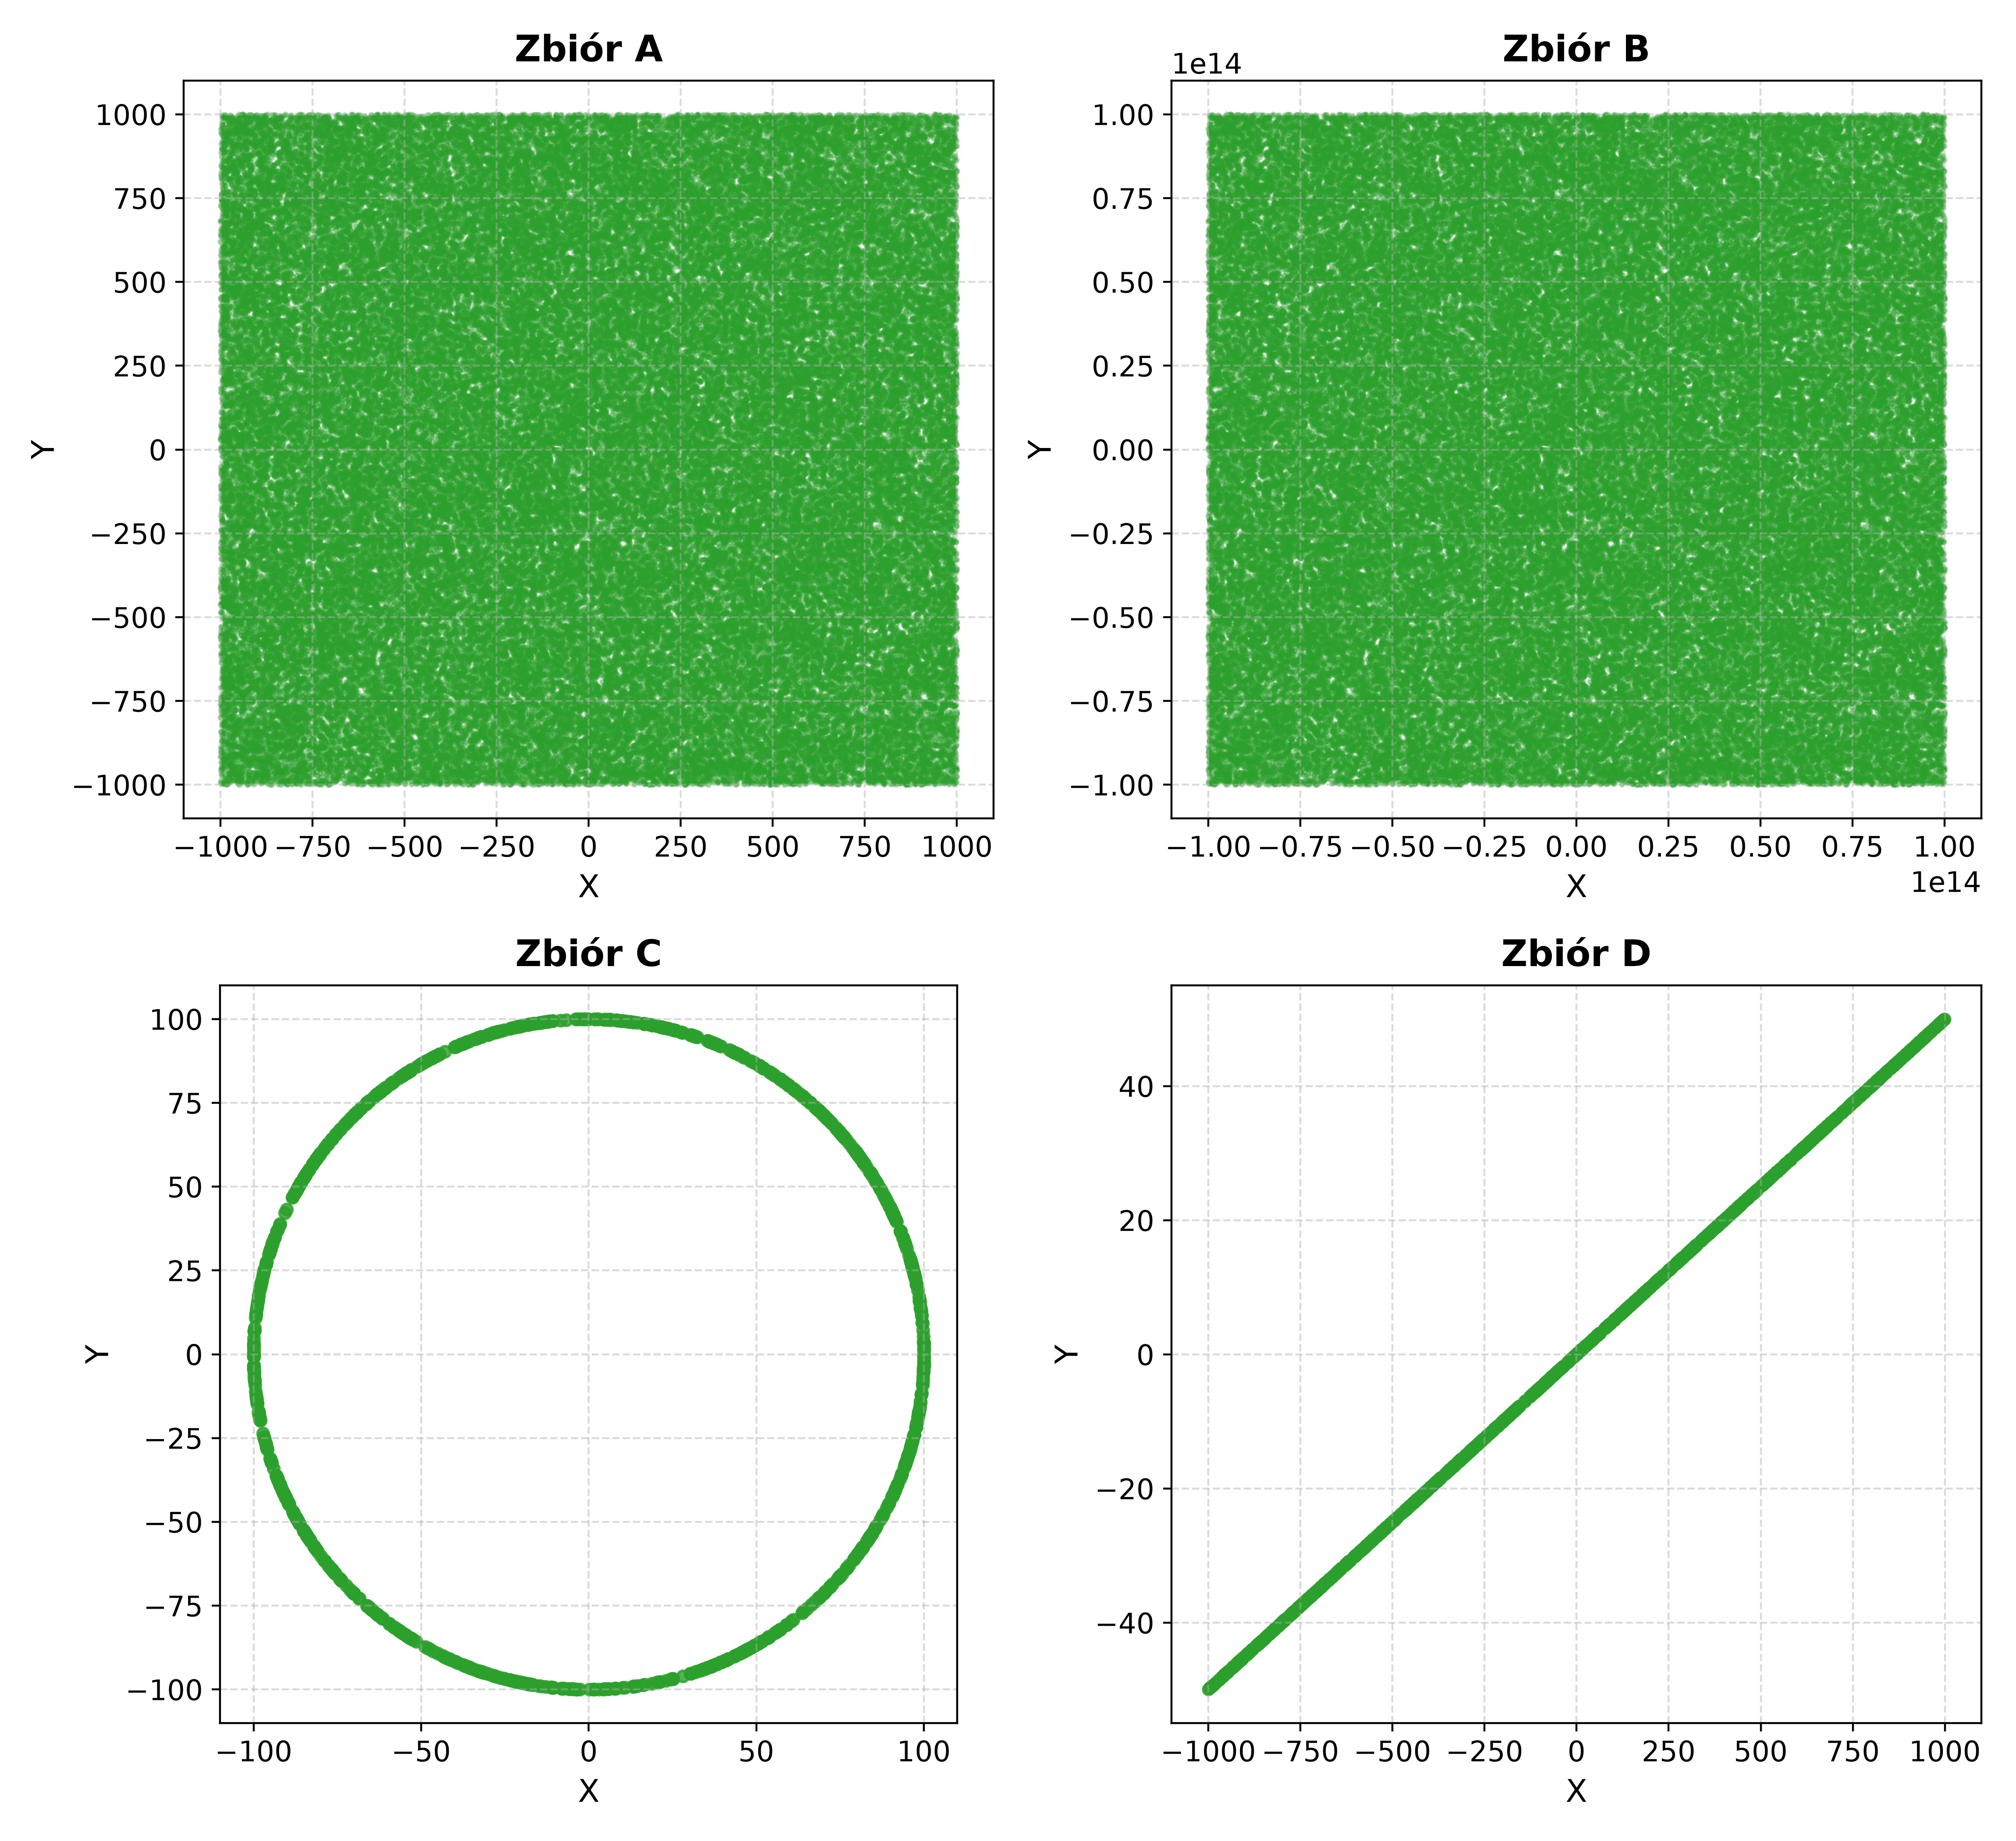
\includegraphics[width=0.68\textwidth]{figures/raw_datasets.png}
    \caption{Wygenerowanie zbiory testowe}
    \label{fig:raw}
\end{figure}

\newpage

\subsection{Wizualizacja klasyfikacji punktów}
Na Rysunku~\ref{fig:classified} zilustrowano podział punktów na kategorie orientacji (Lewo, Prawo, Na prostej) wyznaczony przez prostą $AB$ dla metody \texttt{custom\_2x2} z progiem $\varepsilon = 10^{-10}$.

\begin{figure}[htbp]
    \centering
    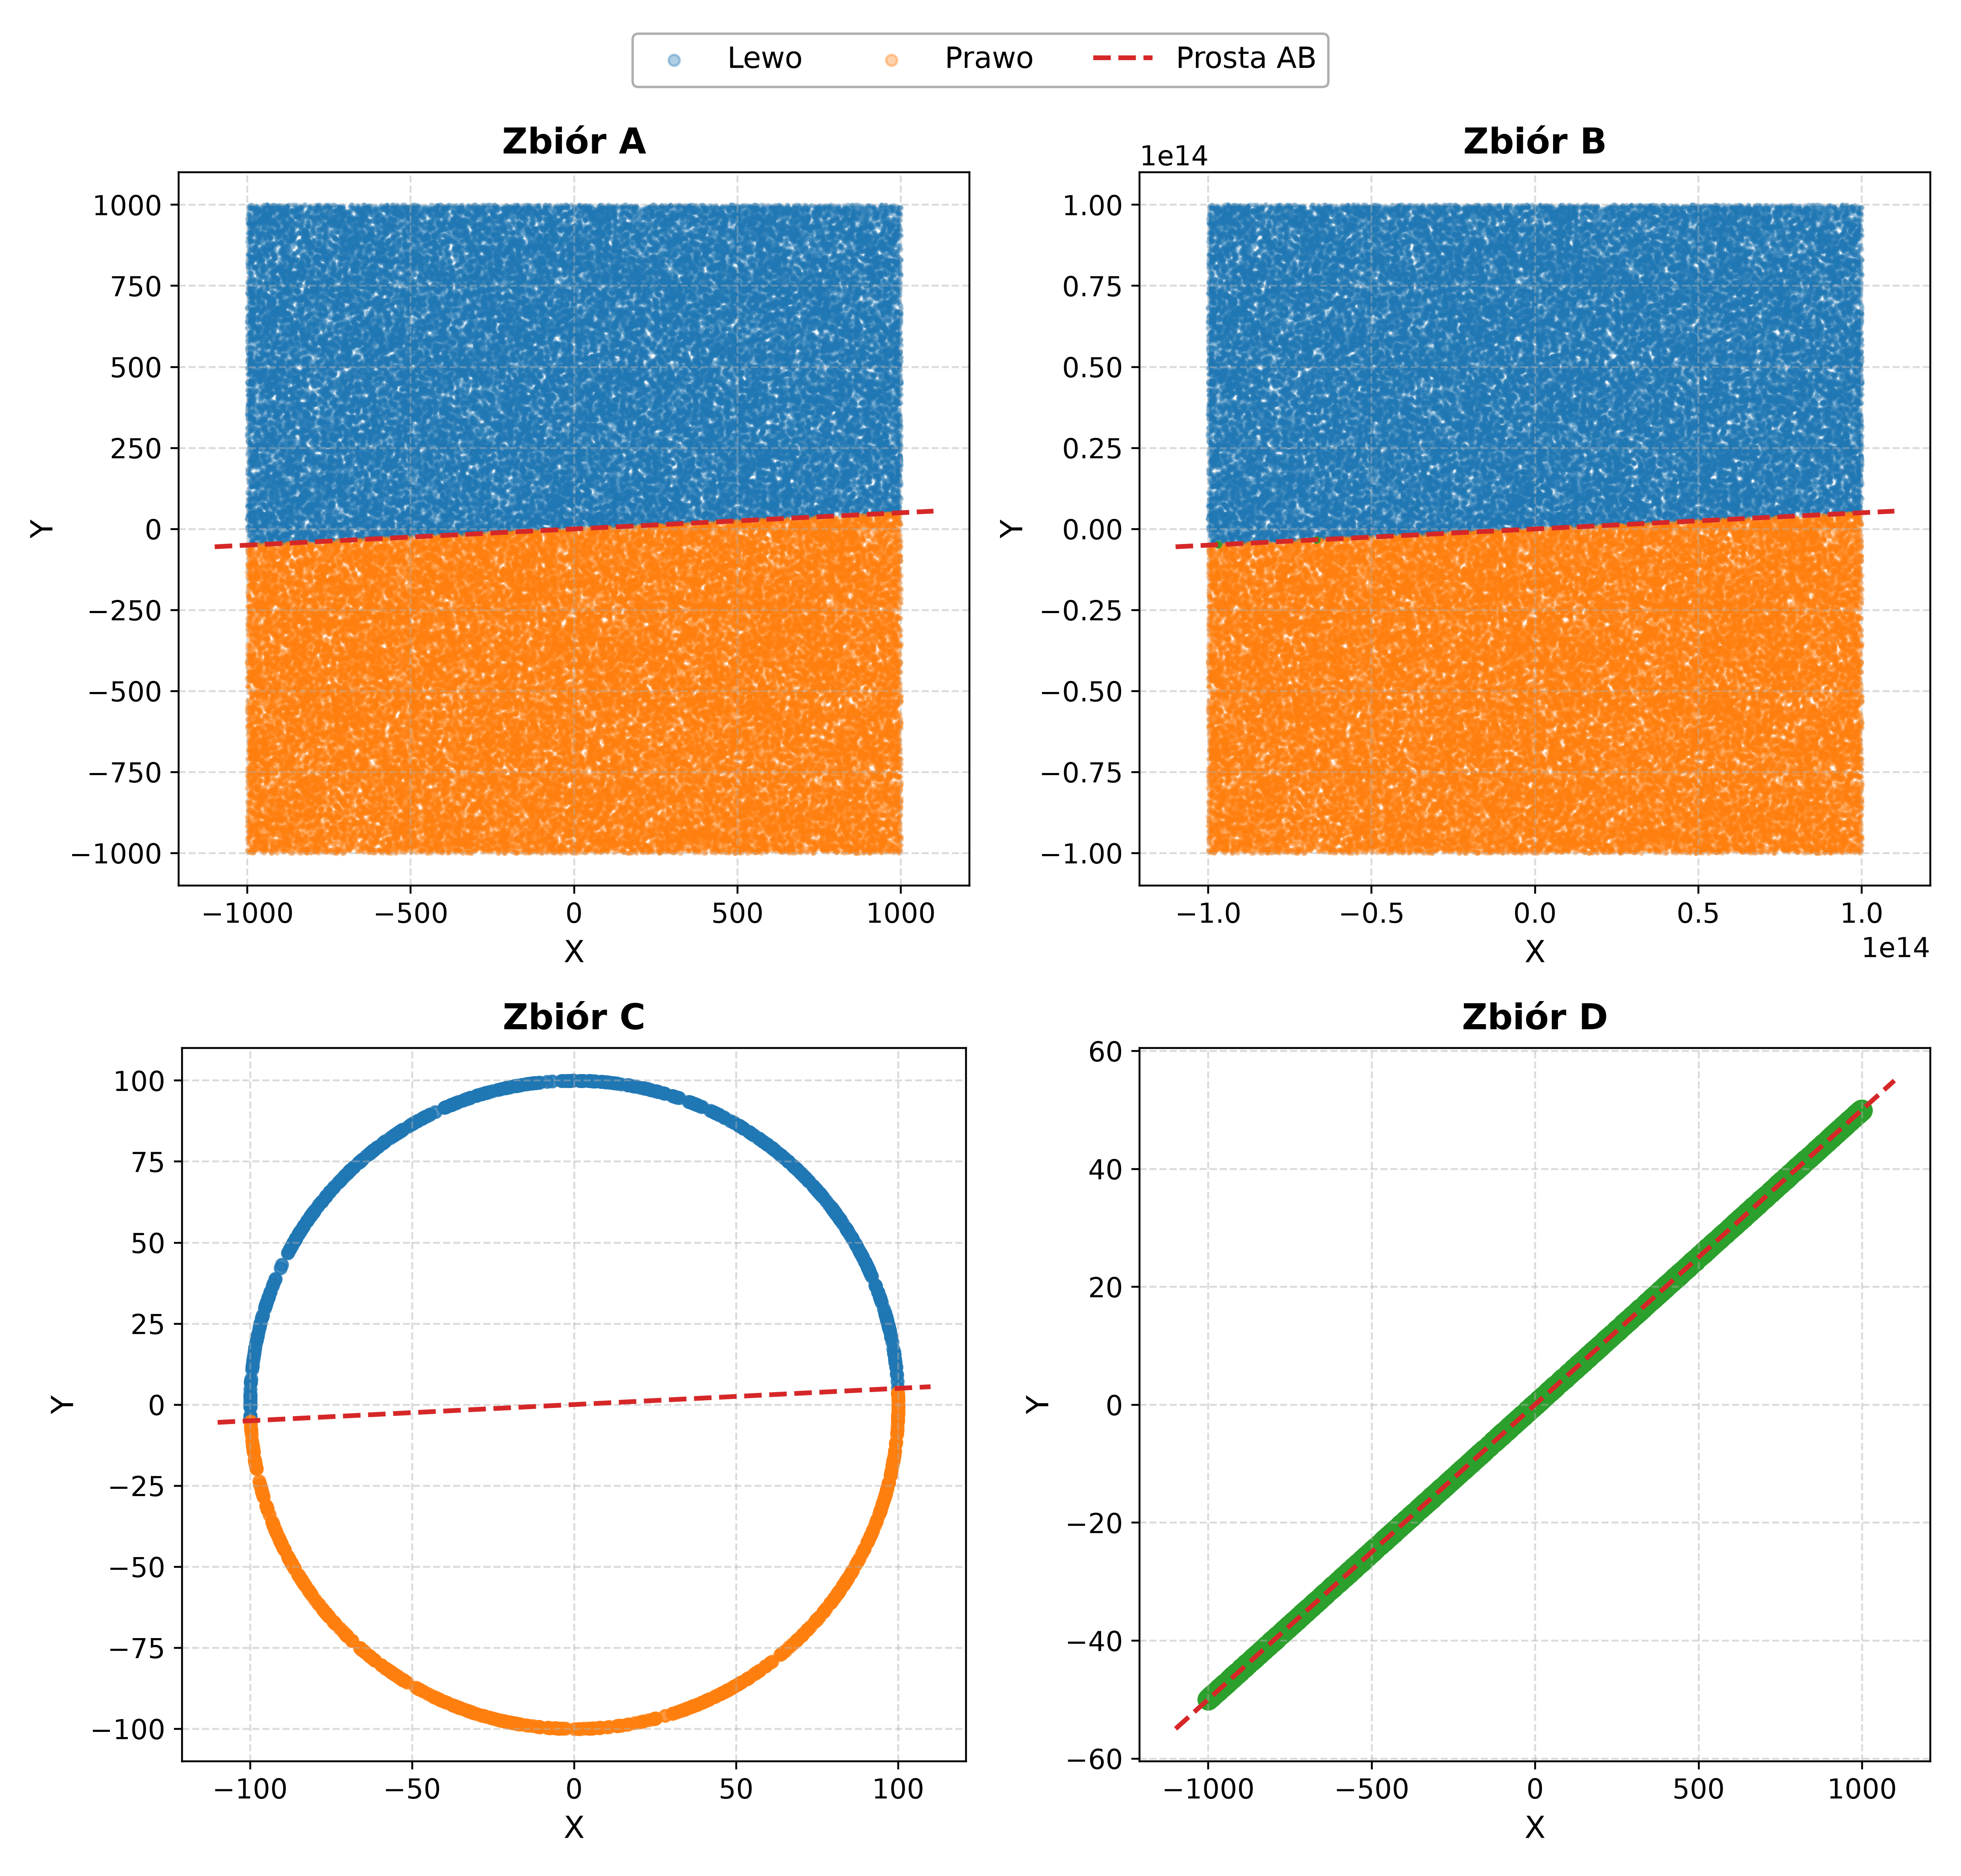
\includegraphics[width=0.64\textwidth]{figures/classified_datasets.png}
    \caption{Klasyfikacja punktów dla wszystkich zbiorów testowych}
    \label{fig:classified}
\end{figure}

\subsection{Wyniki dla zbiorów standardowych (Zbiór A i Zbiór C)}
W tabeli~\ref{tab:set_ac} zestawiono wyniki klasyfikacji uzyskane dla zbiorów A i C. Wyniki te były w $100\%$ identyczne dla wszystkich czterech metod, obu precyzji oraz każdej badanej wartości $\varepsilon$.

\begin{table}[htbp]
\centering
\caption{Stabilne wyniki klasyfikacji dla Zbioru A oraz Zbioru C.}
\label{tab:set_ac}
\small
\begin{tabular}{lcrrr}
\toprule
\textbf{Zbiór} & \textbf{Rozmiar próby} & \textbf{Lewo} & \textbf{Prawo} & \textbf{Na prostej} \\
\midrule
Zbiór A & 100\,000 & 50\,098 & 49\,902 & 0 \\
Zbiór C & 1\,000   & 509    & 491    & 0 \\
\bottomrule
\end{tabular}
\end{table}

\textbf{Wnioski z analizy zbiorów standardowych:}
Dla typowych skal współrzędnych ($[-1000, 1000]$), gdy punkty nie leżą nieskończenie blisko prostej bazowej, wybór metody wyznacznika oraz precyzji nie wpływa na poprawność geometryczną. Wyniki są stabilne i jednoznaczne.

\newpage

\subsection{Zbiór B: Analiza anomalii i fałszywej współliniowości w skali $10^{14}$}
Zbiór B ($10^5$ punktów o współrzędnych rzędu $10^{14}$) ukazuje krytyczne ograniczenia arytmetyki zmiennoprzecinkowej.

\begin{figure}[htbp]
    \centering
    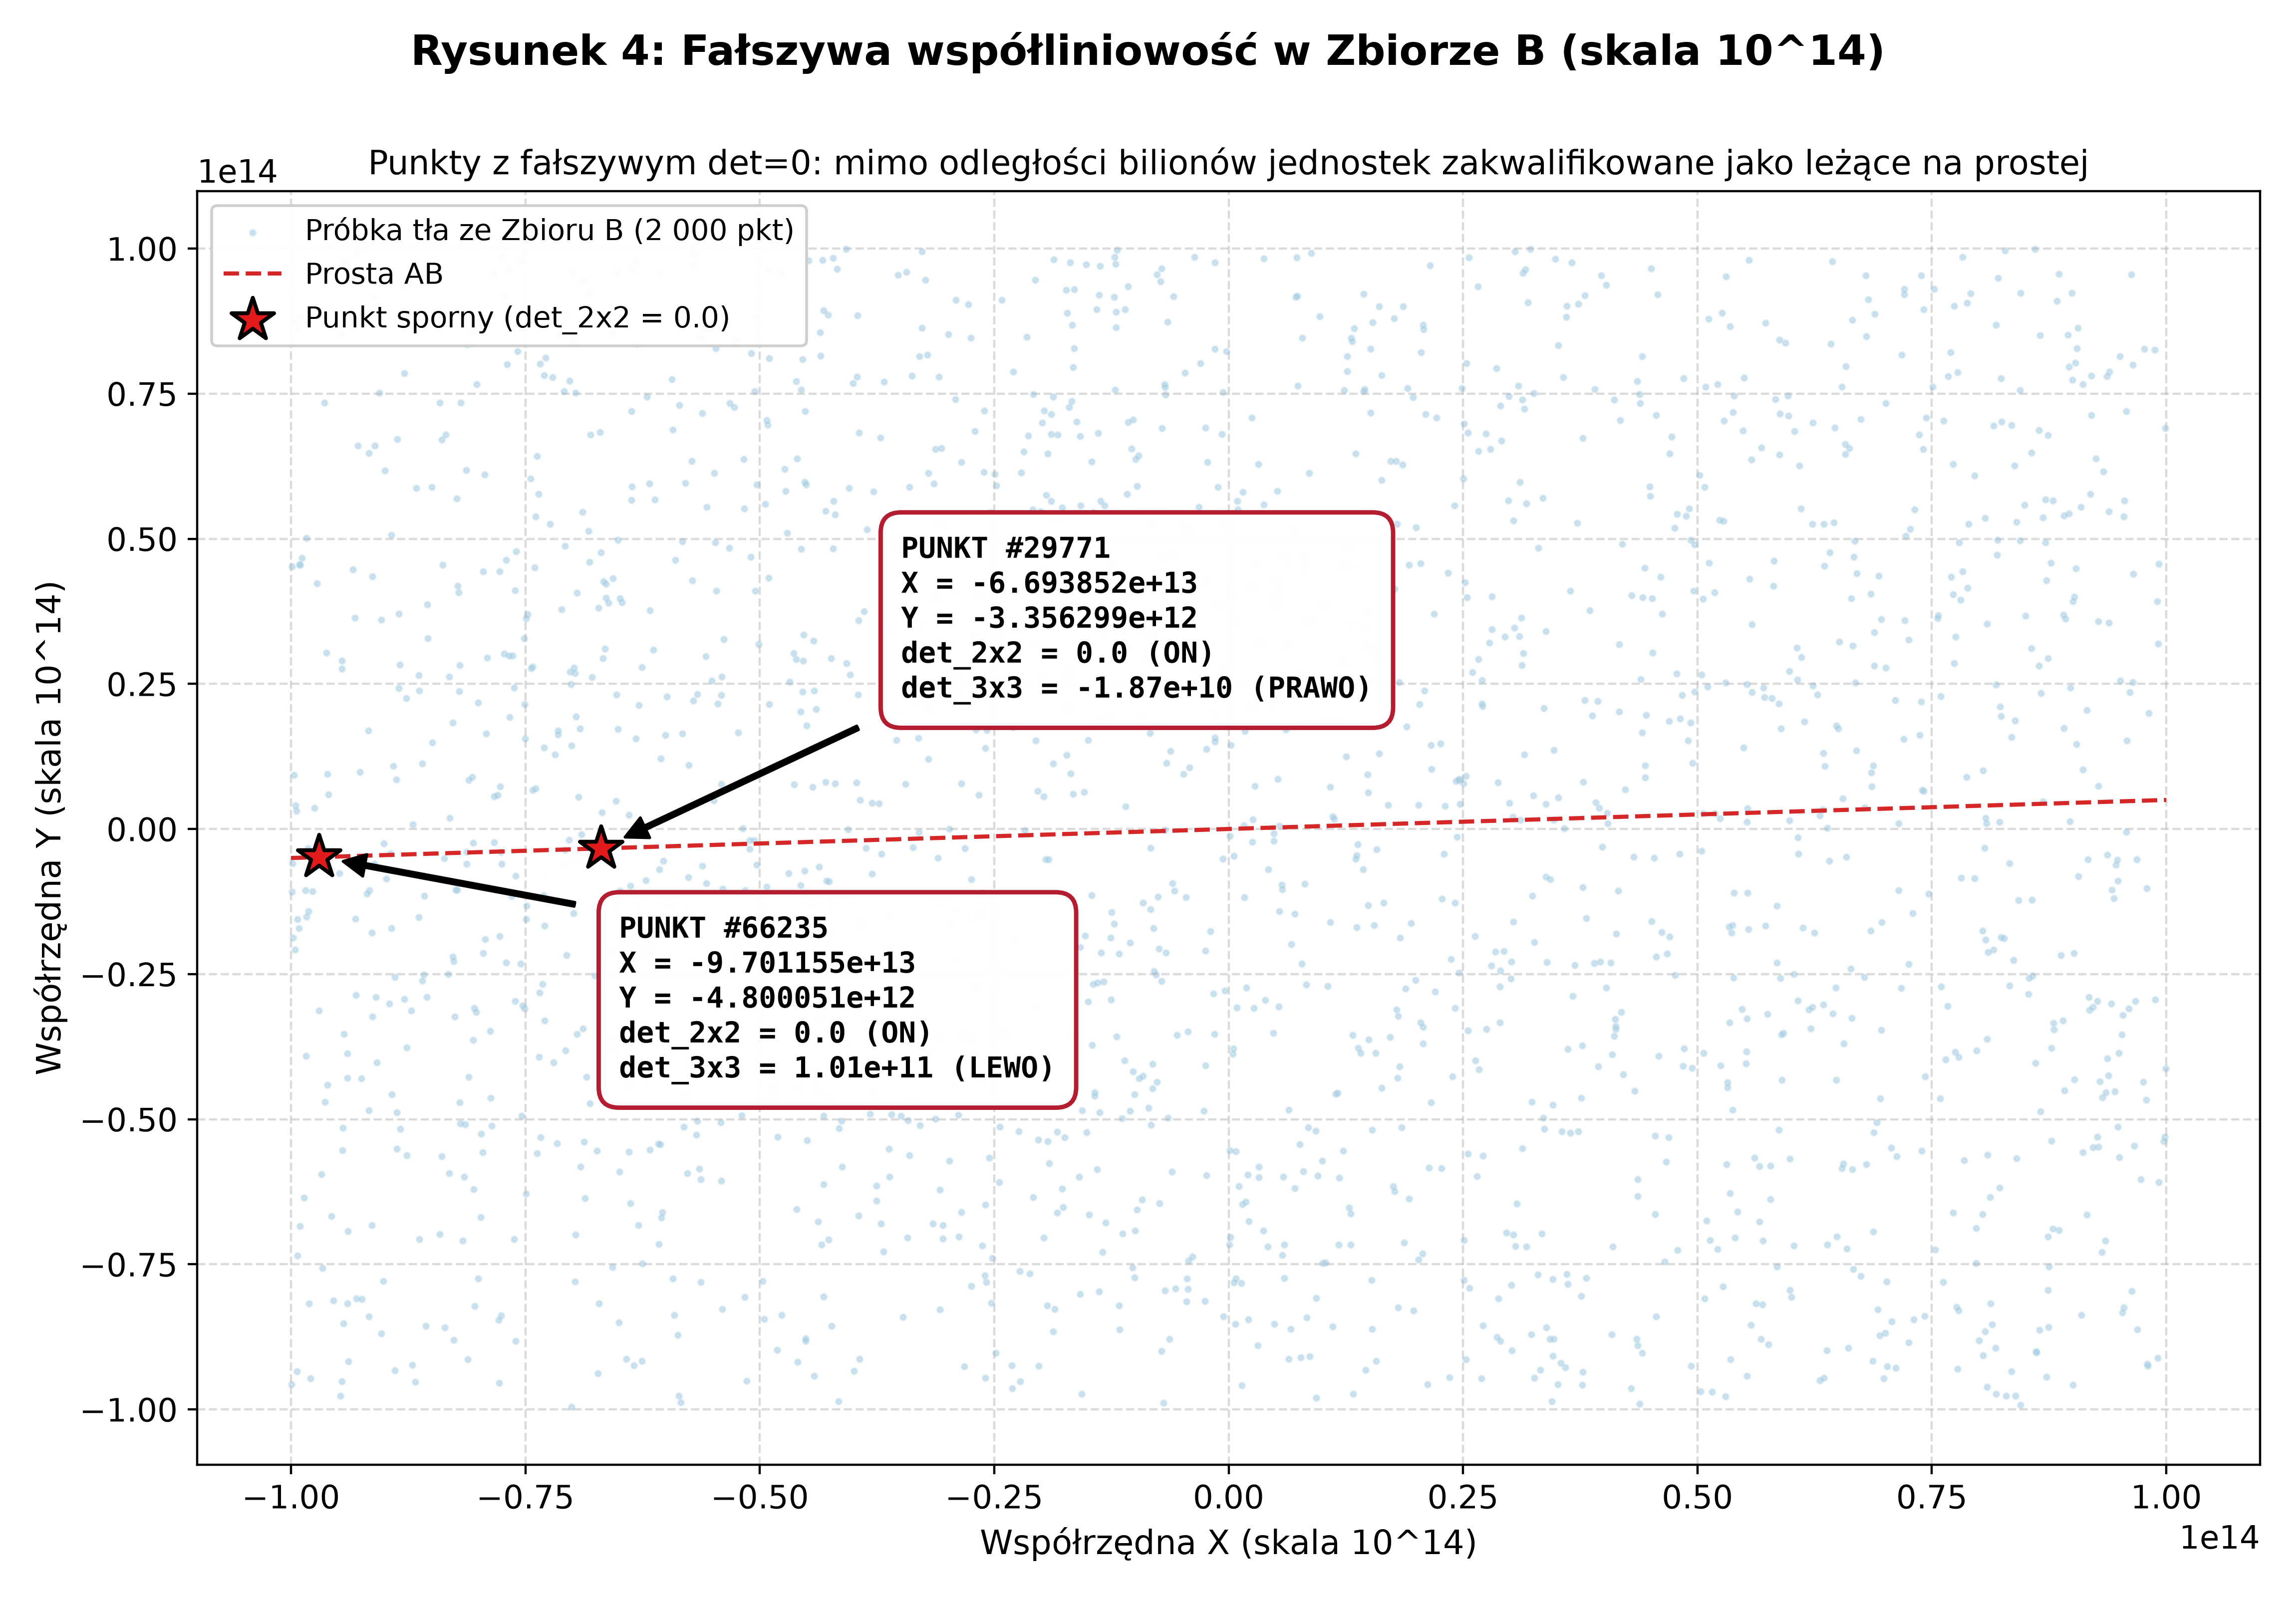
\includegraphics[width=0.75\textwidth]{figures/set_b_anomalies.png}
    \caption{Fałszywa współliniowość w Zbiorze B (skala $10^{14}$) z zaznaczeniem współrzędnych punktów spornych.}
    \label{fig:set_b}
\end{figure}

\begin{table}[htbp]
\centering
\caption{Zestawienie wyników klasyfikacji dla Zbioru B ($10^5$ punktów w skali $10^{14}$).}
\label{tab:set_b}
\small
\begin{tabular}{llcrrrc}
\toprule
\textbf{Metoda} & \textbf{Precyzja} & $\boldsymbol{\varepsilon}$ & \textbf{Lewo} & \textbf{Prawo} & \textbf{Na prostej} & \textbf{Błąd [\%]} \\
\midrule
custom\_3x3 & float64 & 0.0 & 50 098 & 49 902 & 0 & 0.00 \% \\
custom\_2x2 & float64 & 0.0 & 50 097 & 49 901 & \textbf{2} & 0.002 \% \\
numpy\_3x3  & float64 & 0.0 & 50 098 & 49 902 & 0 & 0.00 \% \\
numpy\_2x2  & float64 & 0.0 & 50 098 & 49 902 & 0 & 0.00 \% \\
\midrule
custom\_3x3 & float32 & 0.0 & 50 098 & 49 902 & 0 & 0.00 \% \\
\textbf{custom\_2x2} & \textbf{float32} & \textbf{0.0} & \textbf{0} & \textbf{0} & \textbf{100 000} & \textbf{100.00 \%} \\
numpy\_3x3  & float32 & 0.0 & 50 098 & 49 902 & 0 & 0.00 \% \\
\textbf{numpy\_2x2}  & \textbf{float32} & \textbf{0.0} & \textbf{6 615} & \textbf{6 723} & \textbf{86 662} & \textbf{86.66 \%} \\
\bottomrule
\end{tabular}
\end{table}

\textbf{Analiza anomalii w Zbiorze B:}
\begin{enumerate}
    \item \textbf{Całkowite załamanie \texttt{float32}:} W formule $2 \times 2$ odjęcie małej współrzędnej punktu prostej od liczby rzędu $10^{14}$ powoduje utratę precyzji w 24-bitowej mantysie. Obie różnice stają się numerycznie równe, dając wyznacznik $0.0$ dla całego zbioru ($100\%$ fałszywych współliniowości).
    \item \textbf{Punkty sporne w precyzji \texttt{float64}:} Program zidentyfikował dwa punkty (nr 29771 oraz 66235), dla których \texttt{custom\_2x2} zwrócił dokładnie $0.0$, podczas gdy \texttt{custom\_3x3} dał wyznacznik rzędu $10^{10}$:
    \begin{itemize}
        \item \textbf{Punkt nr 29771:} $X = -6.693852 \times 10^{13}, Y = -3.356299 \times 10^{12}$
        \item \textbf{Punkt nr 66235:} $X = -9.701155 \times 10^{13}, Y = -4.800051 \times 10^{12}$
    \end{itemize}
    Po przeskalowaniu wektora prostej o czynnik $10^{14}$ oba algorytmy uzyskały identyczną wartość $D \approx -10^{27}$ (zgodna klasyfikacja: Prawo). Świadczy to o tym, że błąd wynikał wyłącznie z gigantycznej dysproporcji skali wektora bazowego i badanego punktu.
\end{enumerate}

\newpage

\subsection{Zbiór D: Błędy klasyfikacji na punktach współliniowych}
W Zbiorze D każdy z $1000$ punktów leży matematycznie dokładnie na prostej $AB$. Prawidłowy wynik w idealnej arytmetyce to wyłącznie etykieta Na prostej.

Poniższa tabela przedstawia zachowanie klasyfikatorów w zależności od doboru tolerancji $\varepsilon$ oraz typu danych.

\begin{table}[htbp]
\centering
\caption{Wyniki kategoryzacji punktów Zbioru D (wariant kierunkowy).}
\label{tab:set_d}
\small
\begin{tabular}{llcrrr}
\toprule
\textbf{Metoda} & \textbf{Precyzja} & $\boldsymbol{\varepsilon}$ & \textbf{Lewo} & \textbf{Prawo} & \textbf{Na prostej} \\
\midrule
custom\_3x3 & float64 & 0.0 & 178 & 405 & \textbf{417} \\
custom\_2x2 & float64 & 0.0 & 156 & 156 & \textbf{688} \\
numpy\_3x3  & float64 & 0.0 & 453 & 545 & \textbf{2} \\
numpy\_2x2  & float64 & 0.0 & 503 & 497 & \textbf{0} \\
\midrule
custom\_3x3 & float64 & $10^{-14}$ & 0 & 0 & \textbf{1 000} \\
custom\_2x2 & float64 & $10^{-14}$ & 147 & 147 & \textbf{706} \\
numpy\_3x3  & float64 & $10^{-10}$ & 0 & 0 & \textbf{1 000} \\
numpy\_2x2  & float64 & $10^{-10}$ & 0 & 0 & \textbf{1 000} \\
\midrule
custom\_3x3 & float32 & 0.0 & 298 & 315 & \textbf{387} \\
custom\_2x2 & float32 & 0.0 & 163 & 175 & \textbf{662} \\
numpy\_3x3  & float32 & 0.0 & 489 & 511 & \textbf{0} \\
numpy\_2x2  & float32 & 0.0 & 513 & 487 & \textbf{0} \\
\bottomrule
\end{tabular}
\end{table}

\textbf{Szczegółowa analiza wyników Zbioru D:}
\begin{enumerate}
    \item \textbf{Brak tolerancji ($\varepsilon = 0.0$):} Komputer orzeka poprawną współliniowość zaledwie dla części punktów: 688 w metodzie \texttt{custom\_2x2}, 417 w \texttt{custom\_3x3} oraz zaledwie 0--2 punktów w funkcjach biblioteki NumPy. Wynika to z faktu, że współczynnik prostej $0.05$ jest w systemie dwójkowym ułamkiem nieskończonym okresowym, co przy obliczeniach wyznacznika generuje resztki rzędu $10^{-16}$.
    \item \textbf{Przyczyna rozbieżności między 3x3 a 2x2:} Obie metody wykonują odmienną sekwencję operacji zmiennoprzecinkowych. W formule 3x3 występuje 6 mnożeń pełnych współrzędnych, podczas gdy w 2x2 najpierw odejmowane są współrzędne punktów. Daje to przeciwne znaki resztek wyznacznika, prowadząc do aż 677 sprzecznych decyzji klasyfikatora przy $\varepsilon = 0$.
    \item \textbf{Stabilizacja progiem tolerancji:} Wprowadzenie progu $\varepsilon = 10^{-10}$ całkowicie niweluje wpływ fluktuacji mantysy, przywracając $100\%$ poprawnych orzeczeń (dokładnie $1000$ punktów na prostej) dla wszystkich badanych algorytmów w precyzji \texttt{float64}.
\end{enumerate}

\newpage

\subsection{Porównanie efektywności czasowej (Benchmark)}
Przeprowadzono pomiar czasu klasyfikacji za pomocą \texttt{time.perf\_counter()} dla rozmiarów próby $N \in \{1\,000, 10\,000, 50\,000, 100\,000\}$.

\begin{figure}[htbp]
    \centering
    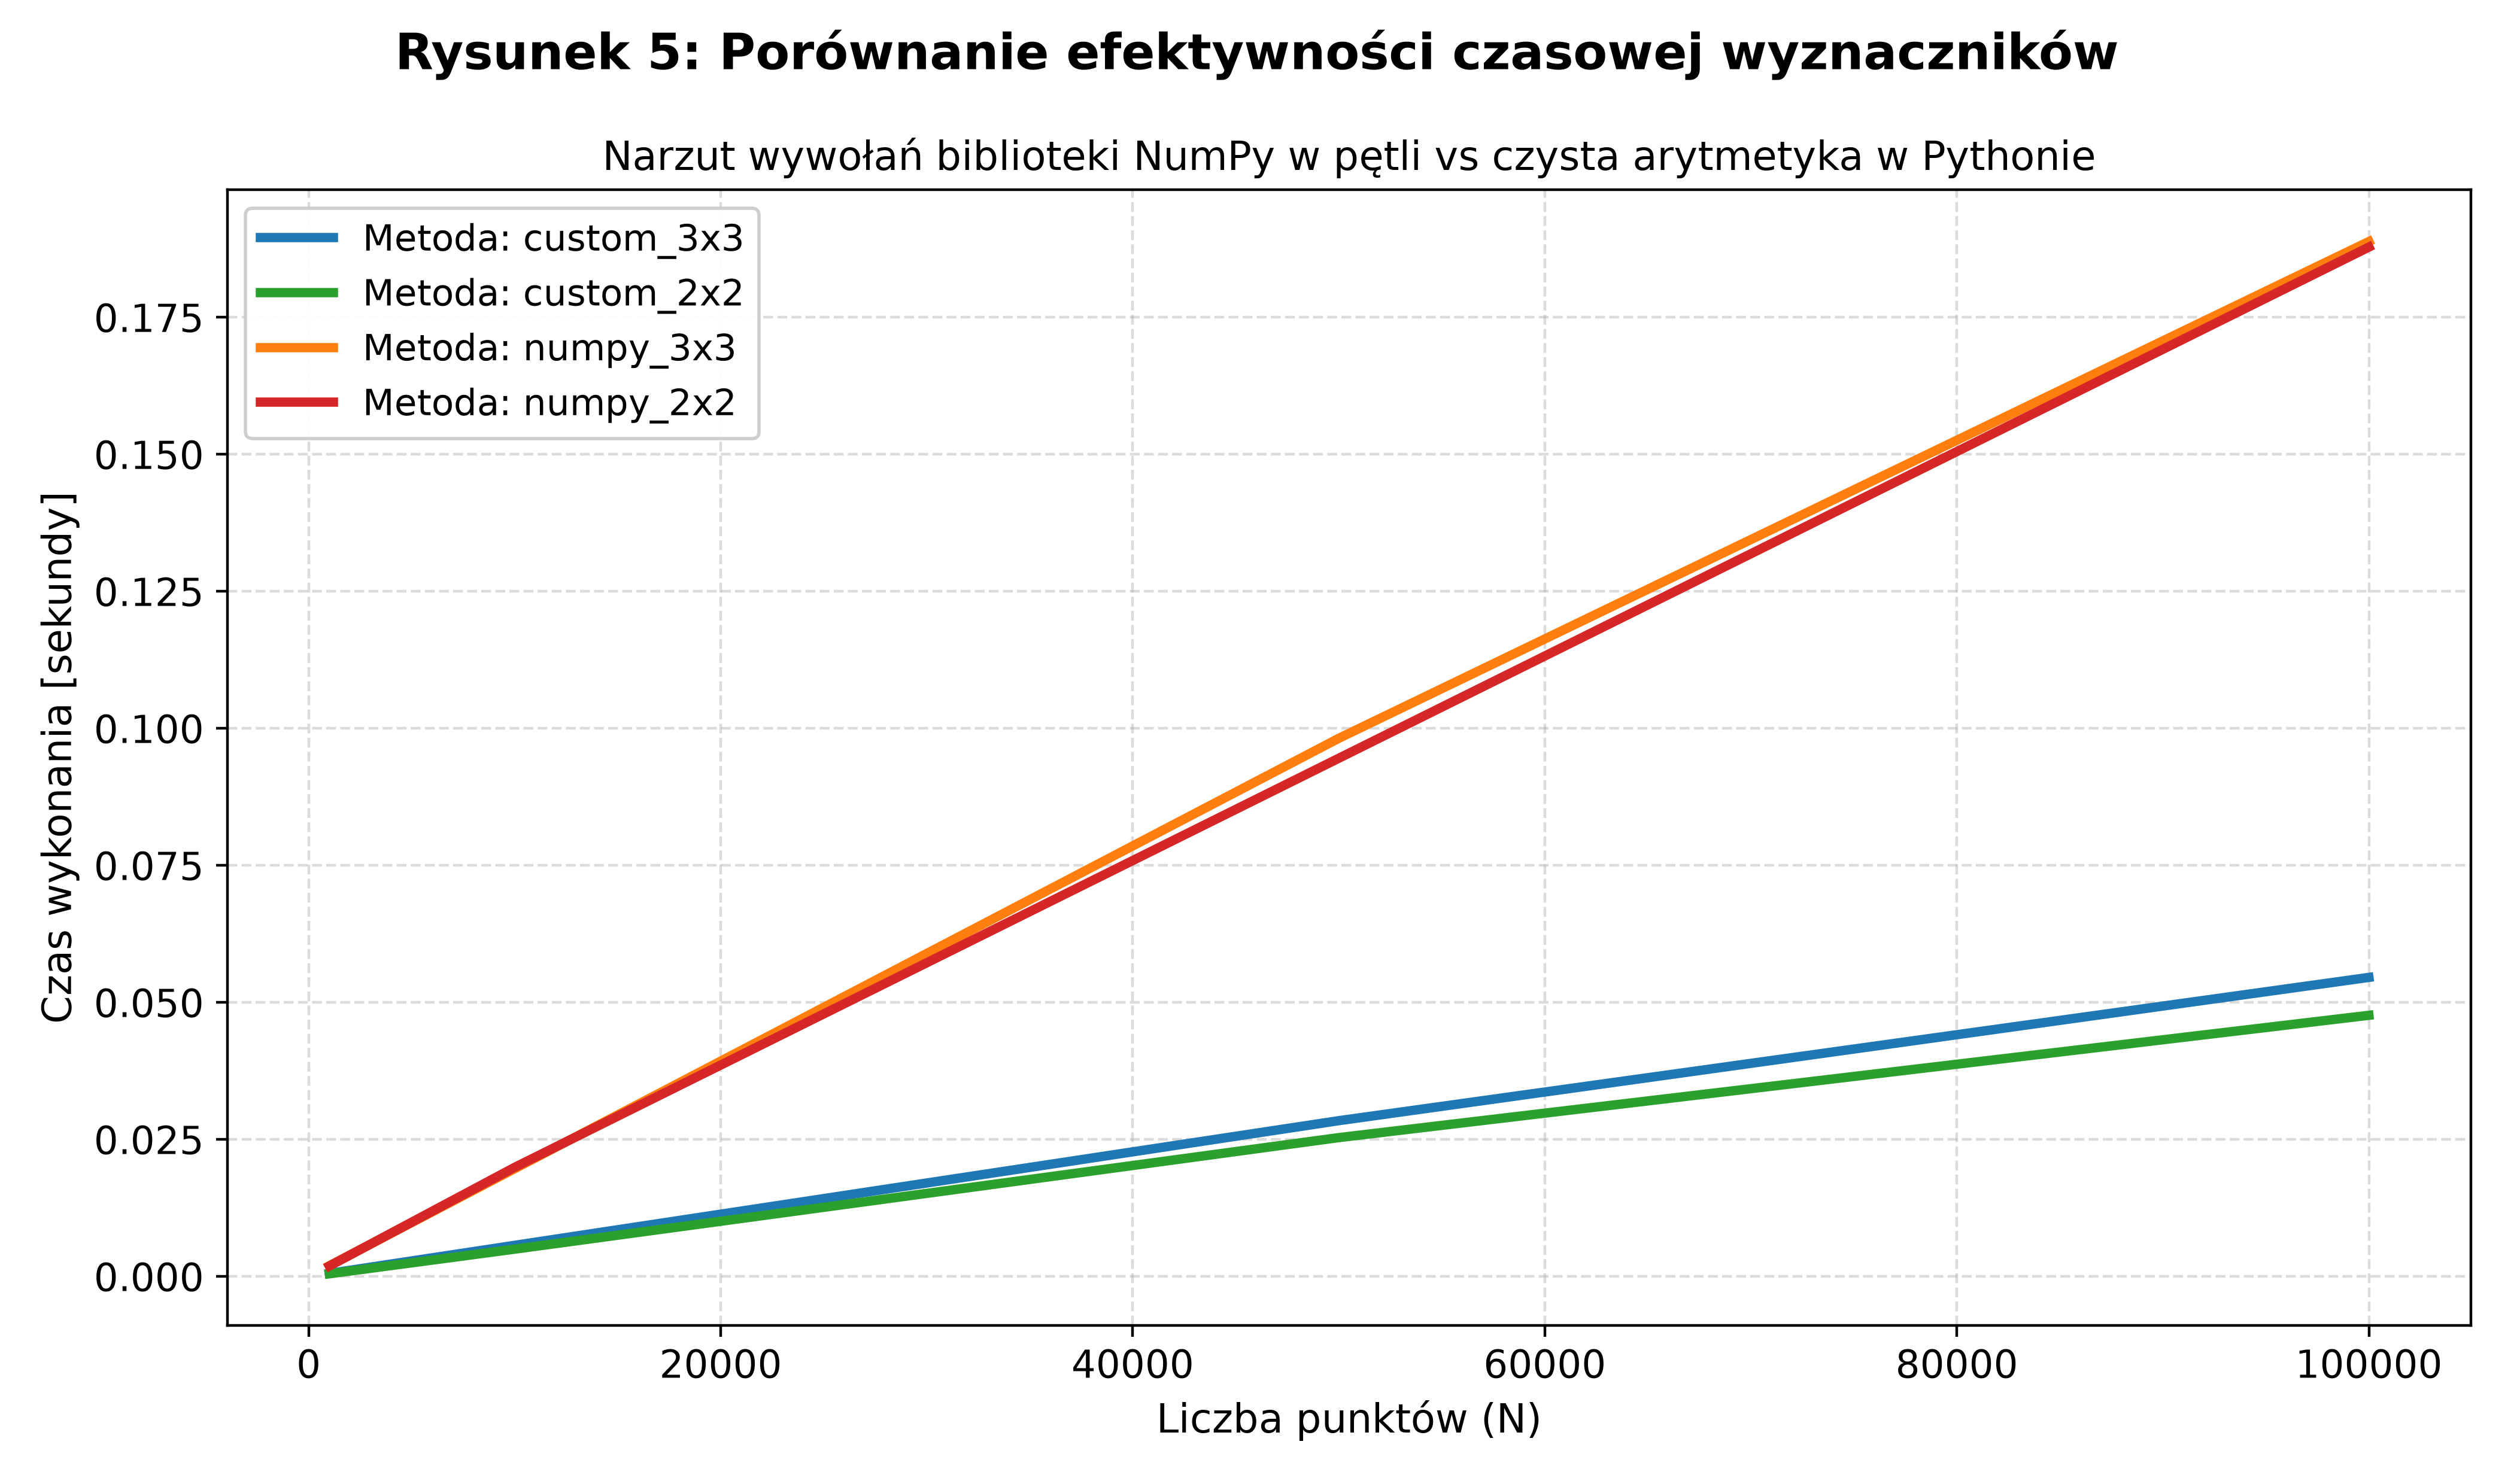
\includegraphics[width=0.75\textwidth]{figures/benchmark_times.png}
    \caption{Zależność czasu wykonania od rozmiaru próby $N$ dla czterech badanych metod.}
    \label{fig:bench}
\end{figure}

\begin{table}[htbp]
\centering
\caption{Średnie czasy wykonania klasyfikacji na procesorze Apple M4.}
\label{tab:bench}
\small
\begin{tabular}{rrrrr}
\toprule
\textbf{Rozmiar próby $N$} & \textbf{custom\_2x2} & \textbf{custom\_3x3} & \textbf{numpy\_2x2} & \textbf{numpy\_3x3} \\
\midrule
1 000   & 0.49 ms  & 0.56 ms  & 1.83 ms  & 1.91 ms \\
10 000  & 4.84 ms  & 5.65 ms  & 18.19 ms & 18.84 ms \\
50 000  & 23.91 ms & 26.96 ms & 88.12 ms & 91.88 ms \\
100 000 & 48.52 ms & 55.41 ms & 179.15 ms & 186.06 ms \\
\bottomrule
\end{tabular}
\end{table}

\textbf{Wnioski z analizy wydajnościowej:}
\begin{enumerate}
    \item Implementacje autorskie (\texttt{custom\_*}) okazały się \textbf{3.4--3.8 raza szybsze} od wywołań biblioteki NumPy w pętli. Dla $10^5$ punktów \texttt{custom\_2x2} wykonuje się w $48.5$ ms, podczas gdy \texttt{numpy\_3x3} wymaga $186.1$ ms.
    \item Narzut NumPy wynika z wywoływania funkcji w pętli \texttt{for} interpretera Pythona --- koszt alokacji obiektów macierzy przewyższa czas samej dekompozycji.
    \item Wszystkie metody wykazują stabilną złożoność liniową $O(N)$.
\end{enumerate}

% --- SEKCJA 5 ---
\section{Wnioski końcowe}
\begin{enumerate}
    \item \textbf{Niewystarczalność formatu \texttt{float32}:} Pojedyncza precyzja nie nadaje się do obliczeń geometrycznych przy współrzędnych powyżej $10^7$. Skutkuje to eliminacją katastrofalną i fałszywym orzekaniem współliniowości na masową skalę ($100\%$ błędu w Zbiorze B).
    \item \textbf{Różnice metod 2x2 i 3x3:} W typowych skalach metoda różnicowa $2 \times 2$ redukuje wielkości operandów i jest stabilniejsza (688 punktów bez tolerancji w Zbiorze D). Jednakże przy braku skalowania wektora bazowego w ekstremalnej przestrzeni ($10^{14}$), odejmowanie małych współrzędnych od ogromnych niszczy informację o nachyleniu prostej.
    \item \textbf{Rola progu tolerancji $\varepsilon$:} Porównanie $D == 0.0$ w arytmetyce zmiennoprzecinkowej jest niepraktyczne. Zastosowanie progu $\varepsilon = 10^{-10}$ dla danych rzędu $10^3$ przywraca pełną $100\%$ zgodność geometryczną we wszystkich badanych metodach.
    \item \textbf{Wydajność implementacji:} Autorska arytmetyka skalarna jest niemal 4-krotnie szybsza od procedur bibliotecznych wywoływanych w pętli \texttt{for}.
\end{enumerate}

\end{document}
